\section{多元统计分析相关基础}
    \begin{enumerate}
        \item
        \code
\begin{lstlisting}
library(ICSNP)
boy <- read.table("data.exam3.4.1.txt", header=TRUE)
mu0 <- c(155,38,2205)
# 取F统计量
HotellingsT2(boy, mu=mu0, test="f")
# 取X^2统计量
HotellingsT2(boy, mu=mu0, test="chi")
\end{lstlisting}
        \out
\begin{lstlisting}
> # 取F统计量
> HotellingsT2(boy, mu=mu0, test="f")

	Hotelling's one sample T2-test

data:  boy
T.2 = 1.3725, df1 = 3, df2 = 26, p-value = 0.2732
alternative hypothesis: true location is not equal to c(155,38,2205)

> # 取X^2统计量
> HotellingsT2(boy, mu=mu0, test="chi")

	Hotelling's one sample T2-test

data:  boy
T.2 = 4.4343, df = 3, p-value = 0.2182
alternative hypothesis: true location is not equal to c(155,38,2205)
\end{lstlisting}
        \summary\\
        $H_0:$数据均值向量等于$(155,38,2205)^{\mathrm{T}}$,$H_1:$数据均值向量不等于$(155,38,2205)^{\mathrm{T}}$,
        \begin{enumerate}[label=(\arabic*)]
            \item 用统计量$F$检验,$p$值为$0.2732>0.05$,则接受原假设,认为数据均值向量等于$(155,38,2205)^{\mathrm{T}}$。
            \item 用统计量$\chi^2$检验,$p$值为$0.2182>0.05$,则接受原假设,认为数据均值向量等于$(155,38,2205)^{\mathrm{T}}$。
        \end{enumerate}
        综上,接受原假设,认为数据均值向量等于$(155,38,2205)^{\mathrm{T}}$。
        \item
        \code
\begin{lstlisting}
A <- matrix(c(0.702,0.541,0.184,0.253,
              0.541,0.712,0.228,0.258,
              0.184,0.228,0.392,0.346,
              0.253,0.258,0.346,0.806), nr=4)
mu0 <- c(22.75,32.75,51.50,61.50)
x0 <- c(22.82,32.79,51.45,61.38)
n <- 21
p <- 4
T2 <- (n-1)*n*t(x0-mu0)%*%solve(A)%*%(x0-mu0);
F <- (n-p)/((n-1)*p)*T2;
pvf <- 1 - pf(F,p,n-p); pvf
\end{lstlisting}
        \out
\begin{lstlisting}
> pvf <- 1 - pf(F,p,n-p); pvf
           [,1]
[1,] 0.03538181
\end{lstlisting}
        \summary\\
        $H_0:\pmb{\mu}=\pmb{\mu}_0,H_1:\pmb{\mu} \neq \pmb{\mu}_0$,$p$值为$0.03538181<0.05$,则拒绝原假设,认为$\pmb{\mu} \neq \pmb{\mu}_0$。
        \item
        \code
\begin{lstlisting}
library(ICSNP)
# (1)
s_ve <- as.matrix(iris[1:100,1:4]);
s_ve_G <- as.factor(iris[1:100,5]);
HotellingsT2(s_ve~s_ve_G)
# (2)
ve_vi <- as.matrix(iris[51:150,1:4]);
ve_vi_G <- as.factor(iris[51:150,5]);
HotellingsT2(ve_vi~ve_vi_G)
# (3)
# setosa
setosa <- as.matrix(iris[1:50,1:4]);
# versicolor
versicolor <- as.matrix(iris[51:100,1:4]);
# vinginica
vinginica <- as.matrix(iris[101:150,1:4]);
n <- 50
p <- 4
avg_s <- as.matrix(colSums(setosa)/50);
avg_ve <- as.matrix(colSums(versicolor)/50);
avg_vi <- as.matrix(colSums(vinginica)/50);
avg <- (avg_s + avg_ve + avg_vi)/3;
A <- 50*(avg_s - avg) %*% t(avg_s - avg) + 50*(avg_ve - avg) %*% t(avg_ve - avg) + 50*(avg_vi - avg) %*% t(avg_vi - avg);
E <- matrix(0,4,4);
for (i in seq(1,n)){
	E = E + (t(t(setosa[i,])) - avg_s) %*% t(t(t(setosa[i,])) - avg_s);
}
for (i in seq(1,n)){
	E = E + (t(t(versicolor[i,])) - avg_ve) %*% t(t(t(versicolor[i,])) - avg_ve);
}
for (i in seq(1,n)){
	E = E + (t(t(vinginica[i,])) - avg_vi) %*% t(t(t(vinginica[i,])) - avg_vi);
}
Lambda <- det(E)/(det(E+A));
pvf3 <- 1-pf((150-3-4+1)/4 * (1 - sqrt(Lambda))/sqrt(Lambda), 8, 2*(150-3-4+1)); pvf3
\end{lstlisting}
        \out
\begin{lstlisting}
> # (1)
> HotellingsT2(s_ve~s_ve_G)

	Hotelling's two sample T2-test

data:  s_ve by s_ve_G
T.2 = 625.46, df1 = 4, df2 = 95, p-value < 2.2e-16
alternative hypothesis: true location difference is not equal to c(0,0,0,0)

> # (2)
> HotellingsT2(ve_vi~ve_vi_G)

	Hotelling's two sample T2-test

data:  ve_vi by ve_vi_G
T.2 = 86.148, df1 = 4, df2 = 95, p-value < 2.2e-16
alternative hypothesis: true location difference is not equal to c(0,0,0,0)

> # (3)
> pvf3
[1] 0
\end{lstlisting}
        \summary
        \begin{enumerate}[label=(\arabic*)]
            \item $H_0:\mu_{setosa}=\mu_{versicolor},H_1:\mu_{setosa} \neq \mu_{versicolor}$,$p$值$< 2.2\times 10^{-16}<0.05$,则拒绝原假设,认为setosa与versicolor的均值向量不相等。
            \item $H_0:\mu_{versicolor}=\mu_{vinginica},H_1:\mu_{versicolor} \neq \mu_{vinginica}$,$p$值$< 2.2\times 10^{-16}<0.05$,则拒绝原假设,认为versicolor与vinginica的均值向量不相等。
            \item $H_0:$三种花的均值向量相等,$H_1:$三种花的均值向量不相等,$p$值为$0<0.05$,则拒绝原假设,认为三种花的均值向量不相等。
        \end{enumerate}
        \item
        \code
\begin{lstlisting}
x <- read.table("ex3_4-data.txt", header=TRUE, row.names=1)
# 均值向量
colMeans(x)
# 协方差矩阵
cov(x)
# 相关系数矩阵
cor(x)
\end{lstlisting}
        \out
\begin{lstlisting}
> # 均值向量
> colMeans(x)
         X1          X2          X3          X4          X5          X6 
 1487.42125   685.85438 10874.18750   449.13000    58.87375    62.83937 
> # 协方差矩阵
> cov(x)
           X1         X2        X3        X4          X5         X6
X1  2093336.6  841893.88  18479476  703207.2  118473.934  139988.10
X2   841893.9  350404.23   7036375  277089.8   48305.919   54154.89
X3 18479475.7 7036374.81 212249748 6910248.0 1017813.524 1424766.40
X4   703207.2  277089.84   6910248  250159.3   38767.802   50785.80
X5   118473.9   48305.92   1017814   38767.8    7008.546    7660.30
X6   139988.1   54154.89   1424766   50785.8    7660.300   10541.30
> # 相关系数矩阵
> cor(x)
          X1        X2        X3        X4        X5        X6
X1 1.0000000 0.9829992 0.8766909 0.9717521 0.9781137 0.9423764
X2 0.9829992 1.0000000 0.8159071 0.9358961 0.9747690 0.8910577
X3 0.8766909 0.8159071 1.0000000 0.9483349 0.8345083 0.9525174
X4 0.9717521 0.9358961 0.9483349 1.0000000 0.9258677 0.9889784
X5 0.9781137 0.9747690 0.8345083 0.9258677 1.0000000 0.8912195
X6 0.9423764 0.8910577 0.9525174 0.9889784 0.8912195 1.0000000
\end{lstlisting}
        \summary
        \begin{enumerate}[label=(\arabic*)]
            \item 数据的均值向量为
            \[(1487.42125,685.85438,10874.18750,449.13000,58.87375,62.83937)^{\mathrm{T}}\]
            \item 数据的协方差矩阵为
            \[\begin{pmatrix}
                2093336.6 & 841893.88 & 18479476 & 703207.2 & 118473.934 & 139988.10 \\
                841893.9 & 350404.23  & 7036375 & 277089.8 &  48305.919  & 54154.89 \\
                18479475.7 & 7036374.81 & 212249748 & 6910248.0 & 1017813.524 & 1424766.40 \\
                703207.2 & 277089.84 &  6910248 & 250159.3  & 38767.802  & 50785.80 \\
                118473.9 &  48305.92 &  1017814  & 38767.8  &  7008.546  &  7660.30 \\
                139988.1 &  54154.89  & 1424766 &  50785.8  &  7660.300 &  10541.30
            \end{pmatrix}\]
            \item 数据的相关系数矩阵为
            \[\begin{pmatrix}
                1.0000000 & 0.9829992 & 0.8766909 & 0.9717521 & 0.9781137 & 0.9423764 \\
                0.9829992 & 1.0000000 & 0.8159071 & 0.9358961 & 0.9747690 & 0.8910577 \\
                0.8766909 & 0.8159071 & 1.0000000 & 0.9483349 & 0.8345083 & 0.9525174 \\
                0.9717521 & 0.9358961 & 0.9483349 & 1.0000000 & 0.9258677 & 0.9889784 \\
                0.9781137 & 0.9747690 & 0.8345083 & 0.9258677 & 1.0000000 & 0.8912195 \\
                0.9423764 & 0.8910577 & 0.9525174 & 0.9889784 & 0.8912195 & 1.0000000
            \end{pmatrix}\]
        \end{enumerate}
        \item
        \code
\begin{lstlisting}
data <- read.table("ex3_4-data.txt", header=TRUE, row.names=1)
x <- data[2:5,]
# 轮廓图
source("outline.R")
outline(x)
# 蛛网图
source("spider.R")
spider(x)
# 调和曲线图
source("harmonic.curve.R")
harmonic.curve(x)
\end{lstlisting}
        \clearpage
        \out
        \begin{figure}[H]
            \centering
            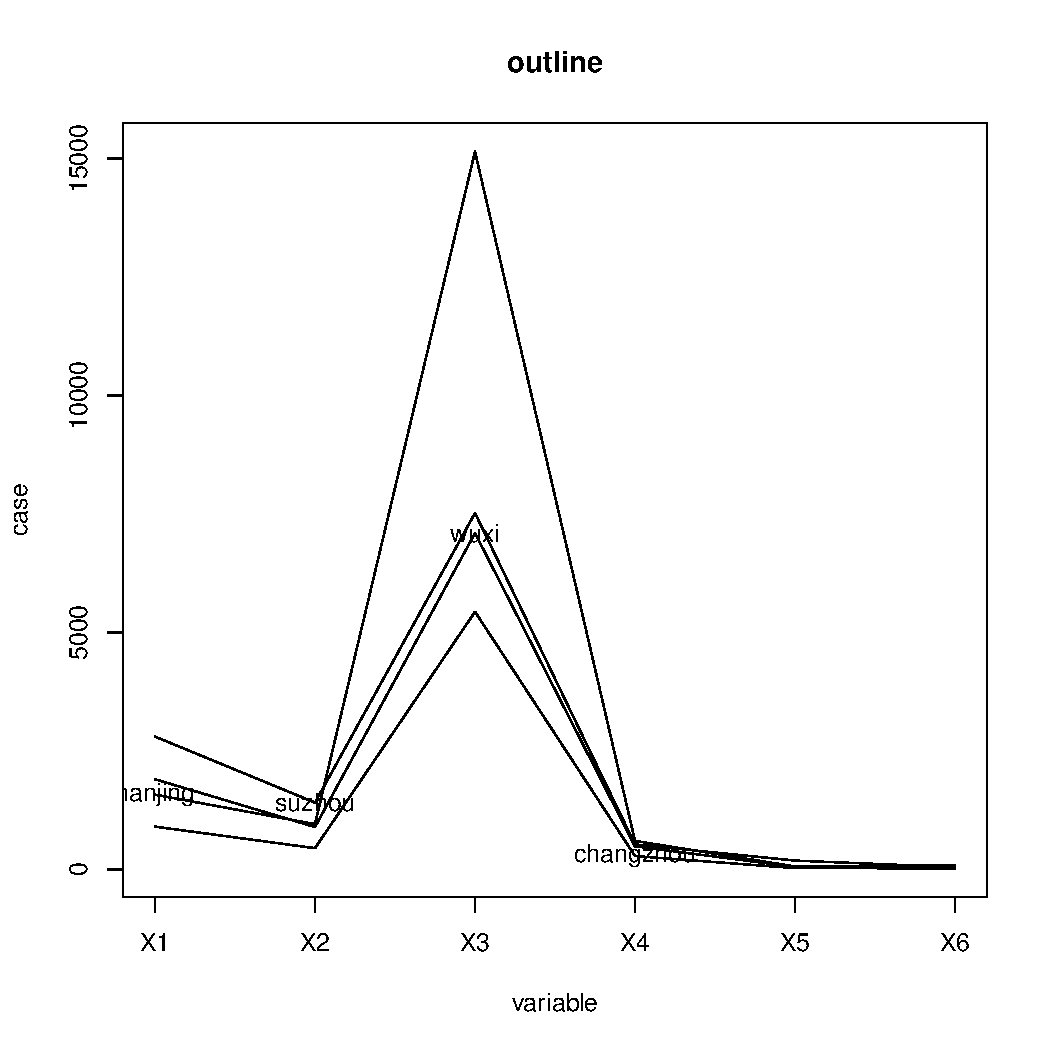
\includegraphics[scale=0.4]{3-5轮廓图.pdf}
            \caption{题5轮廓图}
        \end{figure}
        \begin{figure}[H]
          \centering
            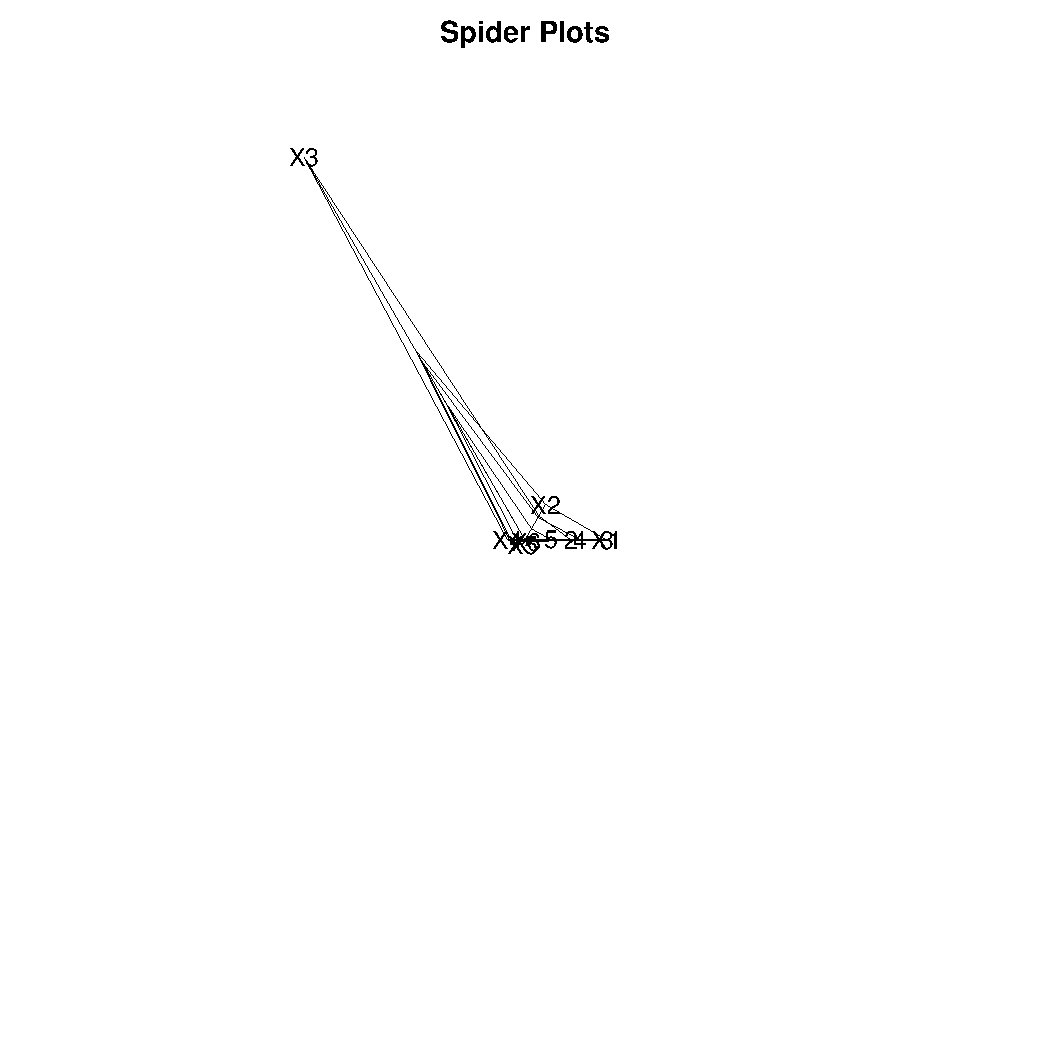
\includegraphics[scale=0.4]{3-5蛛网图.pdf}
            \caption{题5蛛网图}
        \end{figure}
        \begin{figure}[H]
          \centering
            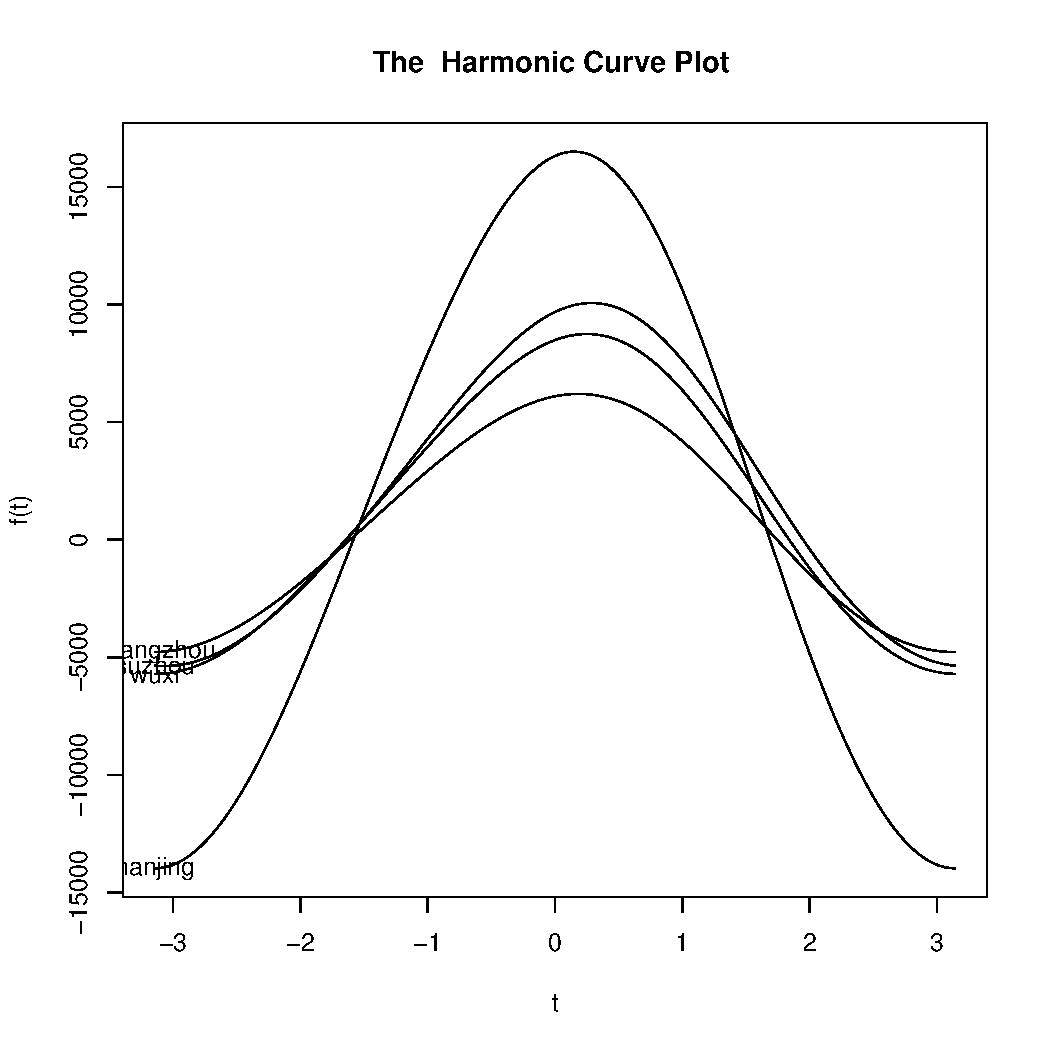
\includegraphics[scale=0.4]{3-5调和曲线图.pdf}
            \caption{题5调和曲线图}
        \end{figure}
    \end{enumerate}
\clearpage